Proteins are complex macromolecules that lie the foundation for all living life on Earth. From providing structural support to cells and tissues through proteins like collagen and keratin, to acting as catalysts for chemical reactions such as the digestion of starch, proteins maintain the normal functioning of living organisms. Since they are fundamental to so many biological processes that make life possible, it is no wonder that the malfunction of proteins can have devastating effects on the health of individuals. To take one example, Parkinson's disease, a chronic degenerative disease that affects the motor system in humans, arises as a result of the aggregation of alpha-sinuclein protein in the brain, a molecule that regulates synaptic vesicle trafficking and subsequent neurotransmitter release.

\section{Computational protein engineering}
Protein engineering is a field of biotechnology that aims to artificially modify existing proteins in order to enhance their properties or create new functions. The field also looks at ways to cure diseases that are the result of malfunctioning biological processes and proteins. For example, as early as 1988, \citet{insulin} induced mutations into the insulin agents used to treat diabetes in order to make them easier to be absorbed by the body and better mimic the action of the naturally-produced insulin hormone. 

Albeit it is a promising field, protein engineering can be a costly, labour intensive process in which researchers have to first determine the mutations most likely to be successful for the task at hand and then experimentally validate them. Moreover, when the discovery process is done experimentally, it may not even be possible, in some cases, to determine the structure of certain unstable proteins. \textit{Computational protein engineering} aims to optimise this exploratory process by using computational methods to accelerate the generation of the most likely to be successful mutations. For example, the last few years have seen a major breakthrough in \textit{protein folding prediction} through the AlphaFold program developed by DeepMind \cite{alphafold}, that uses machine learning (ML) techniques to learn to predict protein structures from their associated sequences. Before AlphaFold, all protein structures would be discovered experimentally in the wet lab over the course of many hours of intensive and expensive labour. With this new computational method, however, researchers can now receive the highly accurate structure prediction of a protein sequence within seconds, thereby making the whole discovery part of the drug design process much faster and efficient. Therefore, computational methods can overcome the limitations of traditional ones by exploring protein structures that have not been experimentally observed yet. 

\section{Equivariant graph neural networks}
This project proposes a novel approach to mutation generation for proteins through the usage of graph neural networks (GNNs). Neural networks are computing systems with interconnected nodes that perform operations on the input data in order to solve a specific task. The nodes' coefficients (commonly called weights) are adjusted by \textit{learning} to approximate functions of the inputs using massive amounts of training examples. Neural networks have become the most widespread approach to machine learning, and are heavily integrated in the fabric of modern society - from content recommendation systems used on social media platforms to language translation and trading on the stock market, almost any digital app can nowadays be augmented with one of the available flavours of neural networks. 

Graph neural networks have gained popularity in the last couple of years and have become the most promising machine learning technique for processing graph information. All GNNs use some form of \textit{neural message passing}, where messages are exchanged between nodes and updated using a neural network \citep{gilmer2017neural}. Many GNNs operate on graphs that represent abstract collections of objects, such as social networks; many, if not all, of the original GNN structures that were proposed would only be able to process scalar features (e.g., in a social network these would be age, gender, social background, etc). However, many real-world graphs are inherently geometric, with nodes having positions in 3D space. To deal with these graphs, the message-passing paradigm was extended to include \textbf{Equivariant Graph Neural Networks} (EGNNs), a type of GNNs that can process information in such a way that preserves the structural properties of the nodes' features. The equivariance and invariance of neural networks, is not, however, a new concept: convolutional neural networks, regarded as the de-facto ML architecture to process image data, already respect the concept of translation equivariance and invariance, as illustrated in Figure \ref{cnn-invariance}. As one can see, a cat stays a cat no matter where it is translated within the picture. 
\begin{figure}
    \centering
    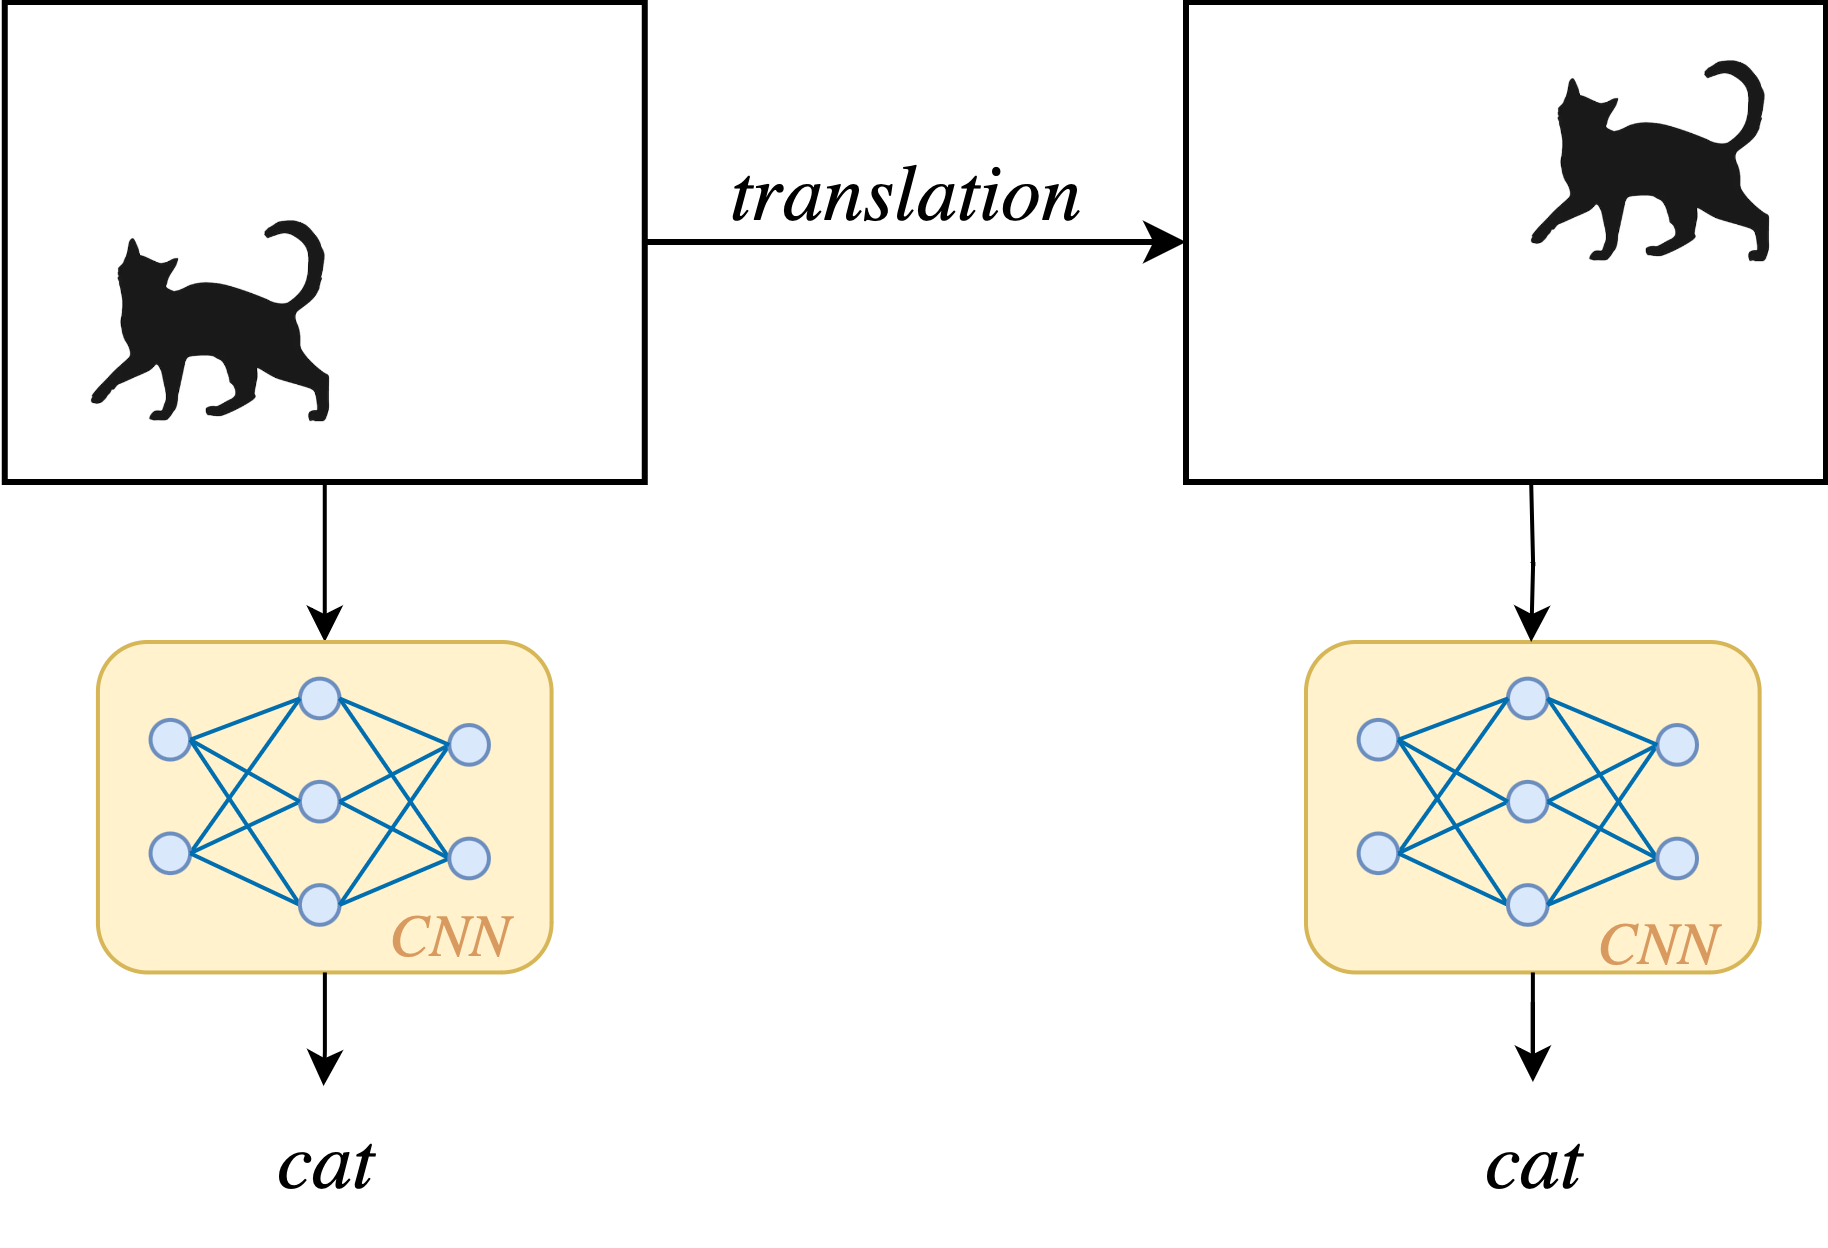
\includegraphics[scale=0.6]{masters-report/figures/cnn-invariance.png}
    \caption{Translation invariance in a CNN.}
    \label{cnn-invariance}
\end{figure}

Protein structures can be represented as graphs with nodes corresponding to atoms. Each atom's scalar feature is its atom type (e.g., Carbon, Nitrogen, Hidrogen, etc.) and its vector feature is the atom's position in 3D space. Using this representation, we can design and train GNNs that are  \textit{equivariant to 3D rotations and translations} to perform a range of molecular tasks. This has approach has already been proven successful on the scoring of protein-ligand complexes \cite{egnn-application-1} or model quality assessment (MQA) \cite{gvp1}.

\section{Unsupervised EGNNs for mutation generation}

The original aim of this project was to evaluate the performance of a handful of newly proposed EGNNs architectures to the molecular task of amino-acid residue identity prediction, also known as the RES task \cite{atom-3d}. This task involves training an ML model to predict the missing amino-acid in a protein given the surrounding atomic environment. 

\textbf{We extend} the original scope of the project to use these trained EGNN models to propose single-point mutations given a protein structure, thereby putting to use the biophysical knowledge that these models have inferred from training on the RES task. These models effectively act as \textbf{unsupervised} models for predicting the \textit{fitness} of a mutated protein, i.e., its ability to perform its biological function more effectively than the wildtype (the non-mutated protein). The idea behind our approach is to use the trained EGNN models to score the existence of a certain amino-acid at a target position in a protein sequence. Figure \ref{idea} illustrates this concept visually. 

\begin{figure}[!h]
    \centering
    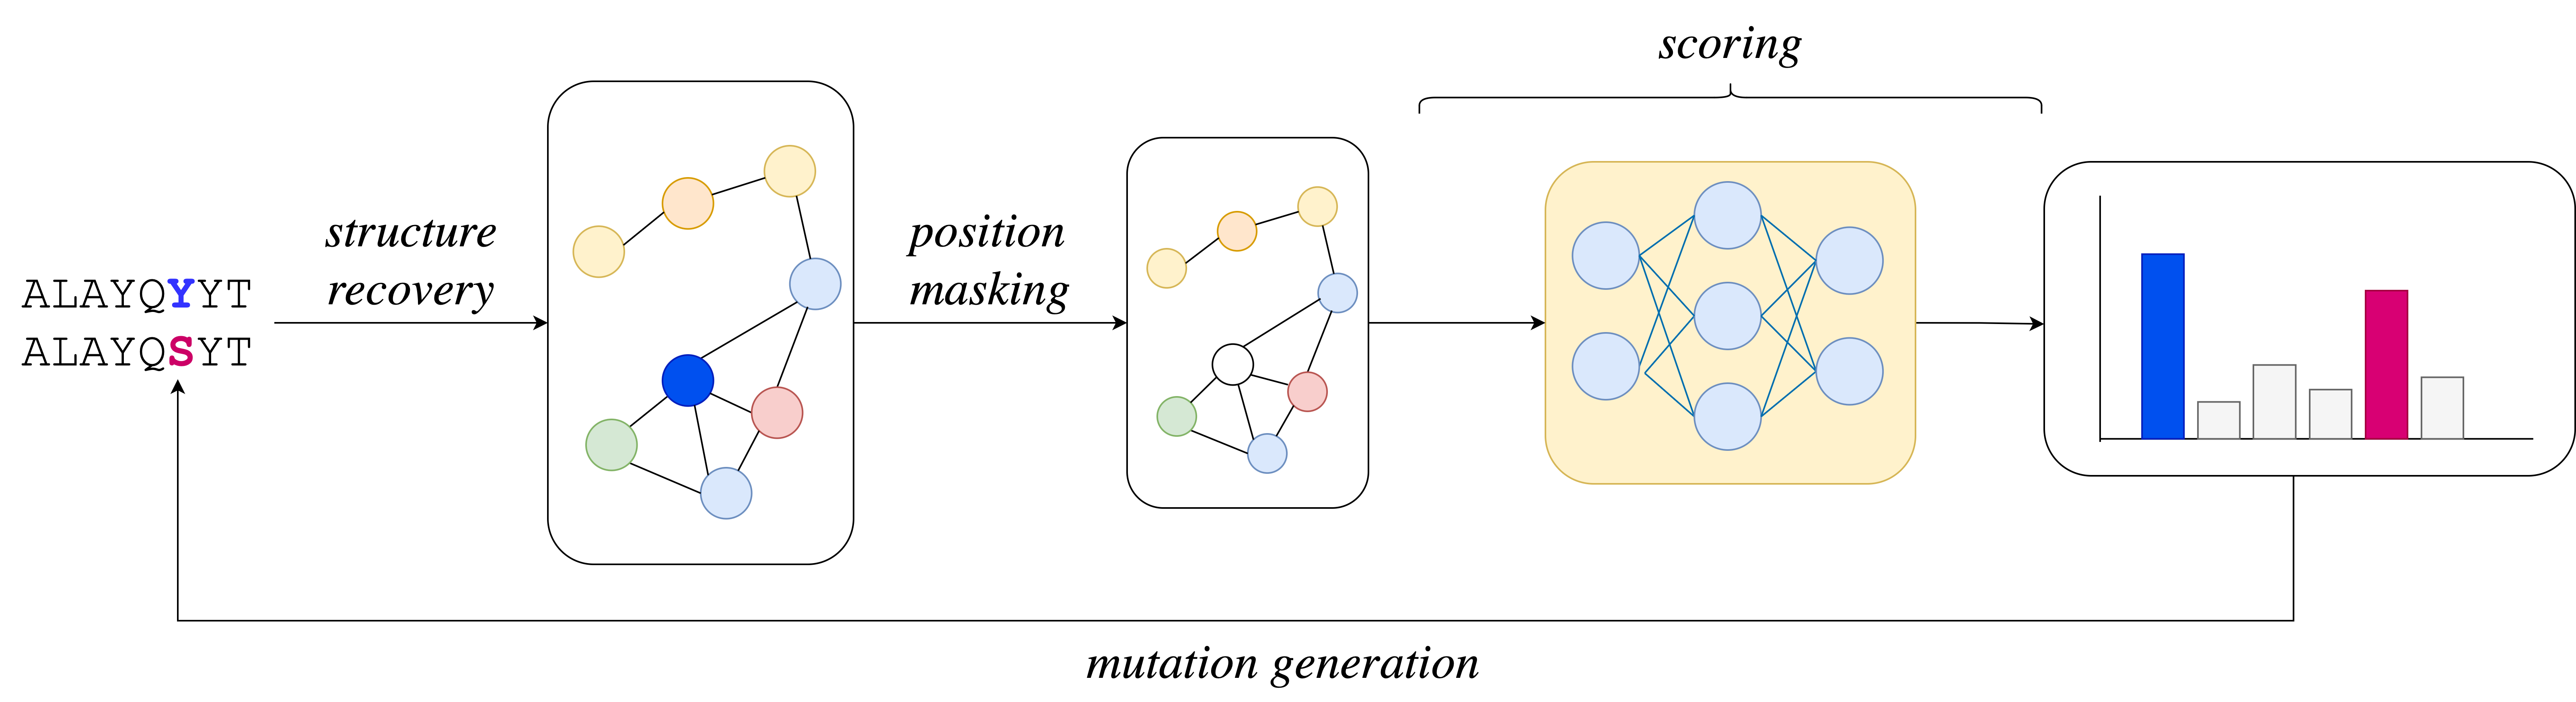
\includegraphics[width=\textwidth]{masters-report/figures/mutation_generation_2.png}
    \caption{The idea behind our mutation generation strategy.}
    \label{idea}
\end{figure}

By targeting each position of an amino-acid sequence in turn, we observe the positions at which the EGNN model is \textit{least confident}. This could be an indication that the position is a good candidate for mutations. Moreover, by looking the scores of all amino-acids at a certain position we can understand what the model thinks are the best matches for that position. The project will compare a couple of systematic approaches for extracting the candidate mutations by looking at both the models' confidence when dealing with amino-acids at targeted positions. 

\section{Augmented linear models for protein fitness prediction}

Having powerful, yet unsupervised models aids the exploratory process when dealing with new proteins – this project acts as a proof-of-concept to how EGNNs can become tools that help researchers accelerate the study of new proteins. Conversely, when data about a mutated sequence's fitness is already available to some extent, we can combine it with the EGNN models proposed in this project in order to create models that effectively operate in a \textbf{low-data regime} and take full advantage of both the latent knowledge of the unsupervised model and the task-specific information provided by the already existing, albeit limited, data. 

To this extent, we propose an \textbf{augmented} ridge regression model that learns to predict the protein fitness of single-point mutated sequences by combining the information about the amino-acid present at each position with the EGNN score for the specified mutation. Although the usage of regression models for fitness prediction was first studied by \citet{chloe-hsu}, we are the first to evaluate this approach using EGNNs and find that it outperforms state-of-the-art transformer models when predicting the fitness of better-than-wildtype sequences. 

\section{Contributions}
